 
\documentclass[conference]{IEEEtran}
%\IEEEoverridecommandlockouts
% The preceding line is only needed to identify funding in the first footnote. If that is unneeded, please comment it out.
\usepackage{cite}
\usepackage[ngerman]{babel}
\usepackage[utf8]{inputenc}
\usepackage{amsmath,amssymb,amsfonts}
\usepackage{algorithmic}
\usepackage{float}
\usepackage{graphicx}
\usepackage{textcomp}
\usepackage{xcolor}
\usepackage{listings}
\usepackage{tabularx}

\bibliographystyle{ieeetr}


\definecolor{pblue}{rgb}{0.13,0.13,1}
\definecolor{pgreen}{rgb}{0,0.5,0}
\definecolor{pred}{rgb}{0.9,0,0}
\definecolor{pgrey}{rgb}{0.46,0.45,0.48}
\lstset{language=Java,
	showspaces=false,
	showtabs=false,
	breaklines=true,
	tabsize=2,
	showstringspaces=false,
	breakatwhitespace=true,
	commentstyle=\color{pgreen},
	keywordstyle=\color{pblue},
	stringstyle=\color{pred},
	basicstyle=\ttfamily
}


\usepackage{url}
\def\BibTeX{{\rm B\kern-.05em{\sc i\kern-.025em b}\kern-.08em
    T\kern-.1667em\lower.7ex\hbox{E}\kern-.125emX}}
\begin{document}

\title{Medizinische Bildverarbeitung - X-Ray Viewer}

\author{\IEEEauthorblockN{Eldin Ramic, Alexander Straube}
\IEEEauthorblockA{\textit{Hochschule München} \\
München, Deutschland \\
e.ramic@hm.edu, straube@hm.edu}
}

\maketitle

\section{Aufgabenstellung}
Im zweiten Laboratorium war das Ziel einen DICOM (Digital Imaging and Communications in Medicine) Volumenbilddatensatz einzulesen, zu verarbeiten und auf unterschiedlicher Art darzustellen.

Zuerst soll ein einzelner Schnitt (Slice) des Datensatzes dargestellt werden, wonach der komplette generierte Volumendatensatz als Gittermodell (Wireframe) angezeigt werden soll. Hierbei ist der Detailgrad des Gittermodells zu hoch und kostet viel Performance, sodass das Deteillevel der Daten zu reduzieren ist.

In der vierten Aufgabe soll der Datensatz mit einer Oberfläche dargestellt und entsprechend beleuchtet werden.

Zuletzt soll der Halterungskäfig aus den Bilddaten entfernt werden, sodass nur noch die Maus zu sehen ist.

\section{Volumenbilddatensatz}

Der gegebene Datensatz umfasst 385 DICOM Dateien, die jeweils Daten, wie das Pixel Array, das Pixel Spacing, Image Position Patient oder andere Header und Meta Informationen, enthalten.

Das Pixel Array ist ein Numpy Array und enthält die Pixel Daten des CT Bildes im Hounsfiled Format. Mit der Hounsfield-Skala wird in der Computertompgraphie (CT) die Abschwächung von Röntgenstrahlung in Gewebe beschrieben und in Graustufenbildern dargestllt. \cite{wiki:HU} \\
Das Pixel Spacing ist der physikalische Abstand im Patienten zwischen der Mitte jedes Pixels, angegeben durch ein numerisches Paar. Diese Information ist wichtig für die Darstellung des Datensatz in einem 3D Gittermodell. \\
Das Image Position Patient Attribut gibt die Bildposition im 3 dimensionalem Raum an. Die x-, y- und z-Koordinaten geben den Mittelpunkt des ersten übertragenen Voxels in der linken oberen Ecke des Bildes an.\cite{pixel_spacing} \\

Im Histogramm \ref{slice_hist} wird die Häufigkeit von bestimmten Hounsfield Units (HU) in allen Bildern des Volumendatensatzes in Relation gesetzt. \\

\begin{table}[ht]
\caption{Substanz - Hounsfiled-Unit Relation}
\centering
\begin{tabular}{|c|c|c|c|c|}
    \hline
	\textbf{Substanz} & \textbf{HU} & \textbf{--} & \textbf{Substanz} & \textbf{HU}\\
	\hline
	Luft & -1000 & -- & Muskeln & +40\\
	\hline
	Fett & -120 & -- & Kontrast & +130\\
	\hline
	Wasser & 0 & -- & Knochen & +400\\
	\hline
\end{tabular}
\label{HU_table}
\end{table}

Das Histogramm \ref{slice_hist} verdeutlicht, dass Pixel mit einem HU von -1000 am Häufigsten vorkommen, was die Substanz Luft repräsentiert. Die Tabelle \ref{HU_table} zeigt die verschiedenen Substanzen, die durch HU definiert werden.

\begin{figure}[H]
	\begin{center}
		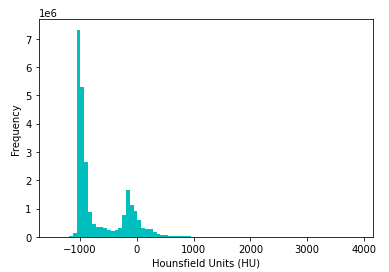
\includegraphics[width=6cm]{latex/images/slices_hist.png}
	 	\caption{Häufigkeit von HU aller Bilddaten}
	 	\label{slice_hist}
	\end{center}
\end{figure}

\section{Einlesen der Daten}
Im ersten Schritt sollen die DICOM Daten aus dem Data-Verzeichnis eingelesen und in entsprechenden Datnestrukturen gespeichert werden.
Mithilfe des Pydicom Python Package\cite{pydicom} können über den Pfad des Data-Verzeichnis alle DICOM Dateien eingelesen, und in einer Liste von FileDatasets gespeichert werden. Dabei wird die Acquisition Number aus den Header Informationen verwendet, um die Schnittbilder in die richtige Reihenfolge zu bringen. \\
Bei der Erstellung einer eigenen Liste mit allen Numpy Arrays, werden die Bilder zusätzlich um 180° gedreht, da ein Fehler bei der Erstellung des Volumendatensatzes auftrat.

\section{Visualisierung der Schnittbilder}
Abbildung \ref{slices} zeigt das Schnittbild an der 150. Stelle im Bilddatensatz auf der linken Seite mit der Colormap "bone" und auf der rechten Seite mit der Colormap "gray".

\begin{figure}[H]
	\begin{center}
		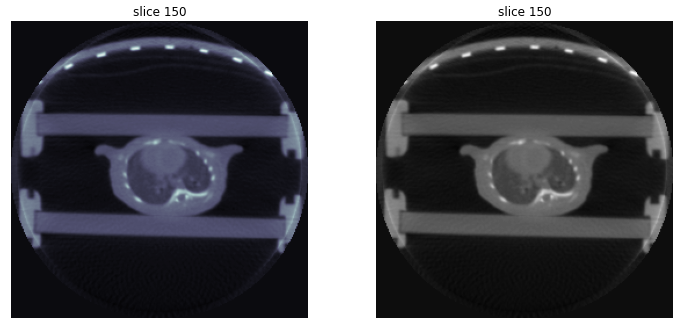
\includegraphics[width=6.5cm]{latex/images/slice_150.png}
	 	\caption{150. Schnittbild des Volumendatensatzes}
	 	\label{slice_150}
	\end{center}
\end{figure}

Abbildung \ref{slices} zeigt neun weitere Schnittbilder des Datensatzes, sodass man eine 3 dimensionale Abbildung einer Maus antizipieren kann.

\begin{figure}[H]
	\begin{center}
		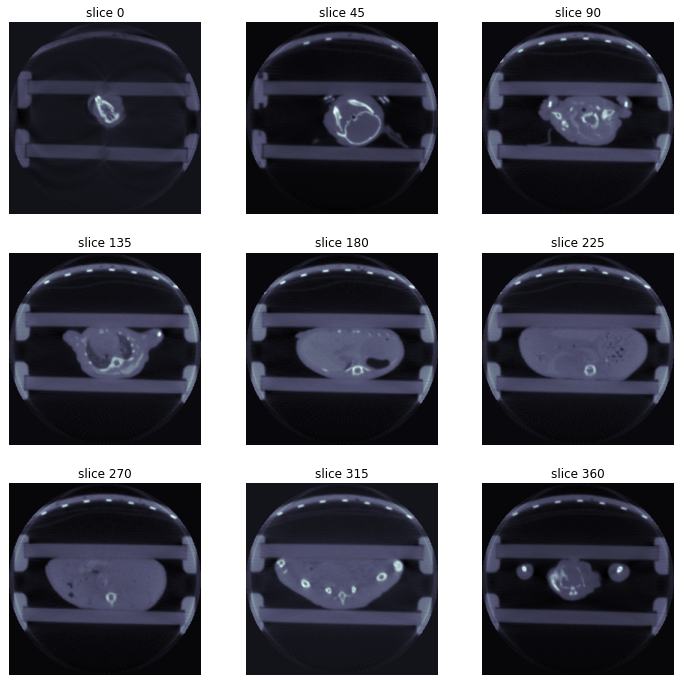
\includegraphics[width=8cm]{latex/images/slices.png}
	 	\caption{weitere Schnittbilder des Volumendatensatzes}
	 	\label{slices}
	\end{center}
\end{figure}

Zusätzlich haben wir eine interaktive Plot Methode implementiert, bei der man über eine Slide-Bar alle Bilder hintereinander anschauen kann. Der zugehörige Code befindet sich im Repository als dicom\_animation Methode.

\section{Darstellen des Volumendatensatzes als Wireframe}
In der dritten Aufgabe ist es das Ziel den Volumendatensatz als Gittermodell anzeigen zu lassen. Dafür gibt es in Python verschiedene Herangehensweisen und Bibliotheken, die auch ein interaktives Gittermodell ermöglichen.
Im ersten Ansatz haben wir über den Marching Cube Algorithmus\cite{marching_cubes} versucht den Volumendatensatz in einem 3D Gittermodell darzustellen. Die skimage und matplotlib Bibliothek bieten die nötigen Funktionalitäten, sodass wir mit den Bilddaten und einem Threshold für die Hounsfield-Unit eine 3D Darstellung erzeugen können. \\
In Abbildung \ref{wireframes} wurde im linken Bild der Threshold auf 700 gesetzt. Da in der Tabelle \ref{HU_table} ein HU Wert ab 400 nur noch Knochen ist, sieht man in dem Bild fast nur das Skelett der Maus. Zudem wurde die facecolor auf weiß und die edgecolor auf blau gesetzt.
Im rechten Bild werden die Oberflächen mit einer anderen Farbe beleuchtet und ein Threshold von 0 wurde gewählt. Dadurch sieht man alle Substanzen ab Wasser nach Tabelle \ref{HU_table} und zusätzlich Ränder des Scans und den Halterungskäfig. Zudem ist besitzt das Modell eine höhere Transparenz. \\

Für das Verständnis für die Rekonstruktion eines 2D Bilddatensatzes mit 3D Volumeninformationen über Pixel Spacing, hat uns ein wissenschaftliche Artikel\cite{3d_reconstructing_dicom} geholfen und kann zum Nachschlagen des Konzepts dienen.


\begin{figure}[H]
	\begin{center}
		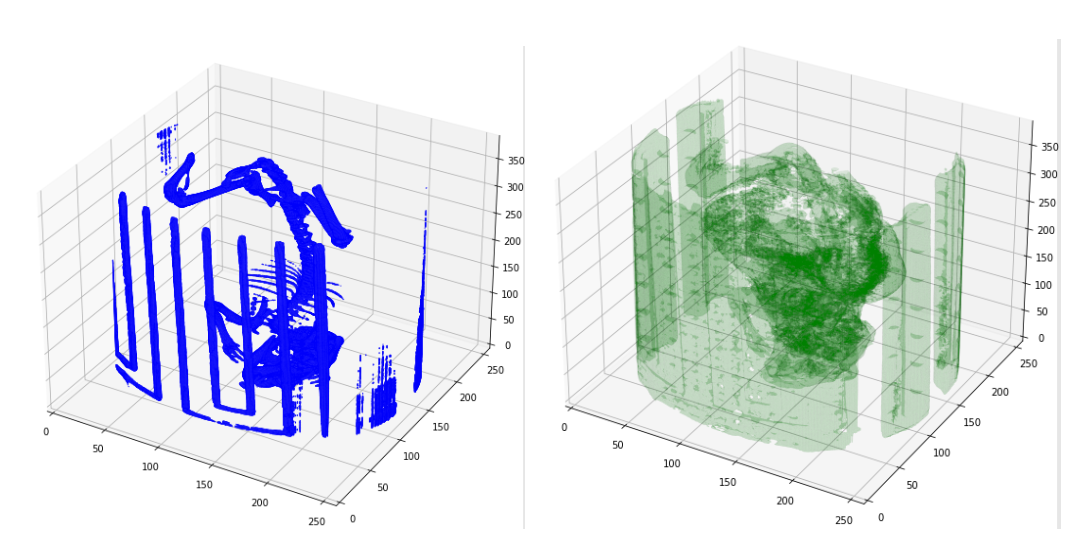
\includegraphics[width=8cm]{latex/images/wireframes.png}
	 	\caption{3D Gittermodell mit unterschiedlichen Thresholds}
	 	\label{wireframes}
	\end{center}
\end{figure}


\section{Darstellen des Volumendatensatzes mit Beleuchtung und Oberfläche}
Das Ziel der vierten Aufgabe war es den Datensatz mit einer Oberfläche darzustellen und diese entsprechend zu beleuchten. Für diese Aufgabe haben wir die SimpleITK Bibliothek\cite{sitk} verwendet, welches ein multi-dimensionales Analyse Toolkit mit sich bringt und Dicom Series in einem interaktiven 3D Gittermodell darstellen kann. \\
Abbildung \ref{sitk_blue_green} zeigt zwei Screenshots von interaktiven 3D Gittermodellen mit unterschiedlicher Parametrisierung. Im rechten Bild wird als Colormap wieder bone verwendet und es ähnelt eher einer 3D Punktwolke. Im rechten Bild werden Oberflächen berechnet und die Beleuchtung wird auf Grün gesetzt.

\begin{figure}[H]
	\begin{center}
		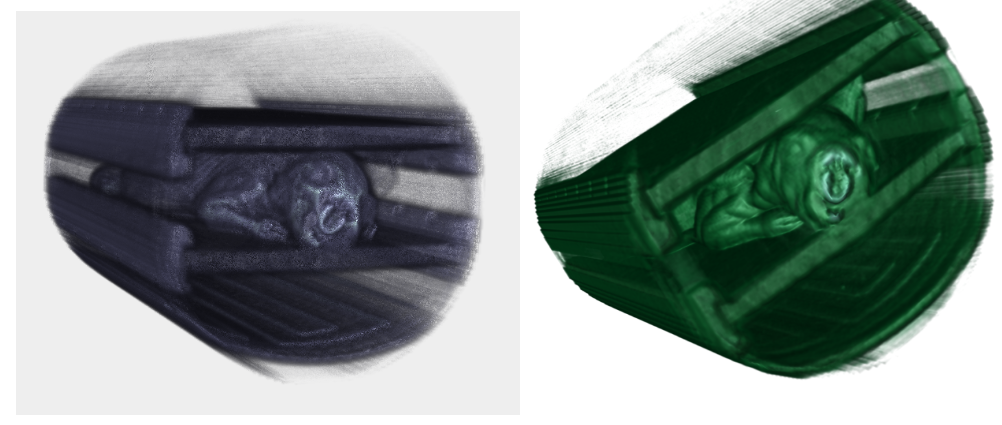
\includegraphics[width=8cm]{latex/images/sitk_blue_green.png}
	 	\caption{Interaktive 3D Gittermodelle mit Oberflächen und Beleuchtung}
	 	\label{sitk_blue_green}
	\end{center}
\end{figure}

Abbildung \ref{sitk_other} zeigt weitere, verschiedene Bilder von der interaktiven 3D Umgebung mit unterschiedlicher/m Beleuchtung, Transparenz, Blickwinkel und Threshold.

\begin{figure}[H]
	\begin{center}
		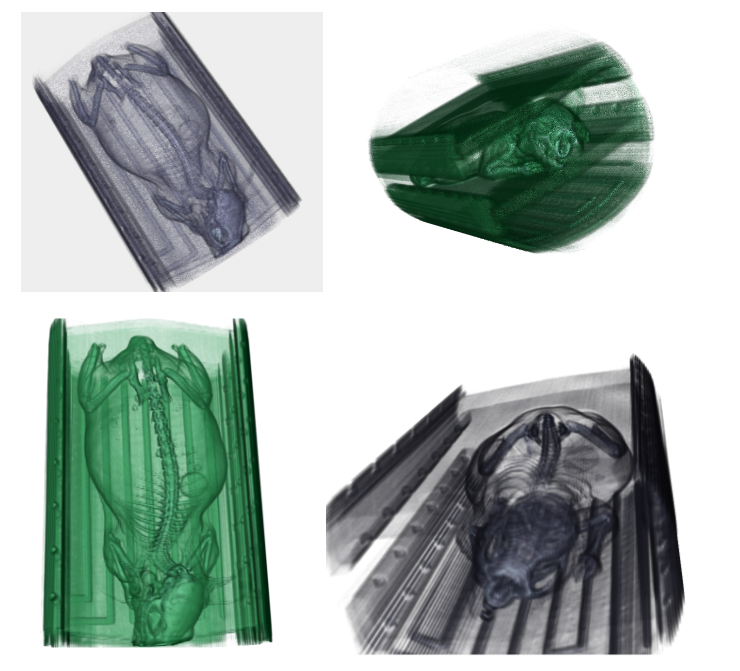
\includegraphics[width=8cm]{latex/images/sitk_other.png}
	 	\caption{Interaktive 3D Gittermodelle mit unterschiedlicher Parametrisierung}
	 	\label{sitk_other}
	\end{center}
\end{figure}


\section{Entfernung des Halterungskäfigs aus den Bilddaten}
In allen bisherigen Bildern ist immer der Halterungskäfig der Maus mit zu sehen. Daher soll in der letzten Aufgabe die Halterung herausgefiltert werden, sodass nur noch die Maus sichtbar ist. Ziel ist es die Pixel zu finden, die zu der Halterung gehören und deren HU Wert auf -1000 zu setzen. \\

Im Folgenden wurde versucht ein Algorithmus zu entwickeln, der alle Dimensionen des Volumens nutzt und nicht nur auf Schnittbilder einer bestimmter Orientierung. Hierbei wurde über eine Ähnlichkeitsmetrik bezüglich der Voxel überlegt, um Voxel mit gleichem oder ähnlichem HU-Wert zu segmentieren. Da die Maus teilweise die gleichen HU-Werte wie der Halterungskäfig hat, werden bei diesem Verfahren auch Teile der Maus mit segmentiert. Aus diesem Grund muss bei der Detektierung des Käfigs auch auf die z-Achse geachtet werden, da der Käfig die breiteste Struktur im Bild und im 3D-Modell ist.
Idee war es anliegende Voxel auf ihren HU-Wert zu analysieren und so entsprechend den Käfig herauszufiltern. Leider hat dieser Ansatz bisher keine verwertbaren Ergbenisse geliefert, sodass wir auf eine andere Herangehensweise gewechselt haben, welche überflüssige Strukturen, wie den Halterungskäfig aus den Bildern entfernt. \\

Der gewählte Ansatz ist nicht sehr dynamisch und statisch auf den gegebenen DICOM Datensatz angepasst. Dabei wurden alle 2D-Bilder durchiteriert, um eine Region of Interest (ROI), die Maus im Zentrum des Bildes, auszuschneiden und in einem eigenem Numpy Array zu speichern. 
Danach muss die ausgeschnittene Maus in ein neu erstelltes Numpy Array mit der selben Dimension, wie die Originalbilder kopiert werden. Das neue Bild besitzt dann die HU-Werte der Maus und alle umliegenden Pixel haben den HU-Wert -1000. In Abbildung \ref{wireframe_no_cage_cut} kann man im Vergleich zu Abbildung \ref{wireframes} erkennen, dass nur noch die Maus sichtbar ist und alle überflüssigen Strukturen, wie der Halterungskäfig, herausgefiltert wurden.

\begin{figure}[H]
	\begin{center}
		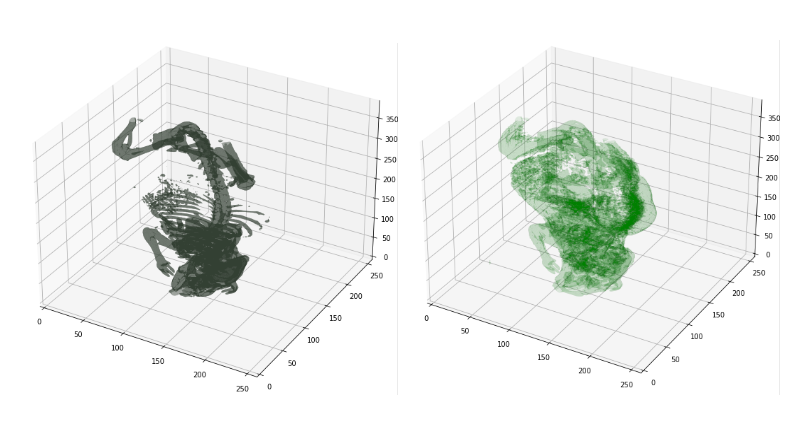
\includegraphics[width=8cm]{latex/images/wireframe_no_cage_cut.png}
	 	\caption{3D Wireframe mit gefilterten Strukturen durch Ausschneiden der Maus}
	 	\label{wireframe_no_cage_cut}
	\end{center}
\end{figure}

In einer letzten Herangehensweise wird versucht die Kanten des Käfigs in den Bildern durch die Hough-Transformation\cite{hough_transformation}, und indirekt durch den Canny-Edge -Detector\cite{Canny-Edge-Detector}, zu bestimmen und danach den HU-Wert auf -1000 zu setzen.
Dafür kann entweder die SimpleITK Bibliothek oder OpenCV herangezogen werden. Um das Ergebnis in einem Gittermodell von Matplotlib darzustellen, haben wir uns für OpenCV entschieden, sodass wir gut mit Numpy Arrays arbeiten können. Wenn  nun noch die zwei vertikale Schnittebenen berechnet werden, ist die Maus ausgeschnitten und alle Voxel um die Maus herum haben den HU-Wert -1000. Abbildung \ref{wireframe_no_cage_cut} zeigt das Ergebnis.

\section{Optimierungsmöglichkeiten und Erweiterungen}
Der Volumenbilddatensatz wurde erfolgreich eingelesen, verarbeitet, visualisiert und der Halterungskäfig entfernt. Hier liegt auch das größte Optimierungspotential, da die Eliminierung hauptsächlich über die 2-dimensionalen Bilder stattgefunden hat. Hier könnten weitere und effizientere Verfahren zur Segmentierung oder Eliminierung entwickelt werden. Man könnte beispielsweise ein Neuronales Netz darauf trainieren die Halterung und alle weiteren überflüssigen Strukturen aus dem Volumenbilddatensatz zu entfernen.


% \section{Programmiersprache, Programm Architektur, Entwicklungsumgebung}

\bibliography{literature}

\end{document}